\documentclass{article}
\usepackage[utf8]{inputenc}
\usepackage{relsize, amsmath}
\usepackage{amsfonts}
\usepackage{amsthm}
\usepackage{enumitem}
\usepackage{graphicx}
\usepackage{amssymb}
\usepackage[export]{adjustbox}
\usepackage[T2A]{fontenc}
\usepackage[russian]{babel}
\usepackage{hyperref}
\hypersetup{
	colorlinks=true,
	linkcolor=blue,
	filecolor=magenta,      
	urlcolor=cyan,
}

\usepackage[left=1.8cm,right=1.8cm,top=1.7cm,bottom=1.7cm,bindingoffset=0cm]{geometry}

\title{Отчёт по работе над дипломным проектом}
\author{Хусаинов Анвер M3439}

\begin{document}
	\maketitle
	\begin{center}
		Отчёт №2 (18.11.19 – 12.12.19)
	\end{center}

	
	Цель спринта: найти устойчивые метрики при применении метода \href{https://arxiv.org/abs/1701.01140}{Regularized IV} во множестве "случайных" экспериментов. \\
	
	Перед описанием основной цели спринта отмечу, что был модифицирован метод из предыдущего отчёта, который состоял из оптимизации функции, содержащей слагаемыми с изменёнными, неизменёнными результатами и результатами AA-тестирования. Однако в следствие этого возникло несколько гиперпараметров, от значений которых сильно зависела сходимость метода, максимизирующего функцию. Таким образом, этот метод в силу своей экспериментальности, сложности обучения и отсутствия реальных AA-данных отложен до лучших времён. \\
	
	Метод из основной части спринта также был упомянут в предыдущем отчёте, вкратце его можно описать так: применение линейной регрессии с регуляризацией на короткие метрики по p-value (незначительные изменения --- ставим 0). Также я добавил l2-регуляризацию в качестве ещё одной степени свободы метода (первая -- значение p-value, по которому отсекать).
	
	Был пересчитан график из первого отчёта по значению MSE при удалении доли выбросов. Проблема с предыдущим заключалась в том, что выбросы удалялись из тест-сета тоже, из-за чего MSE увеличивалась. Реальный график показан на рисунке \ref{fig:mse_nu}. Этот график строился без регуляризации. Из него я сделал вывод, что очистку шума можно вести с долей не выше, чем 0.2.  \\

	\begin{figure}[h]
		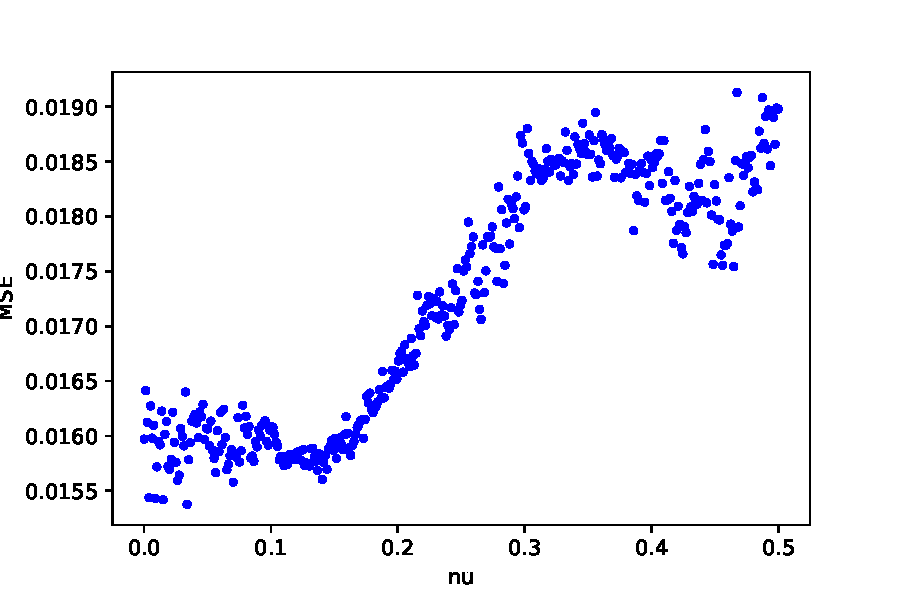
\includegraphics[scale=1]{MSE_nu_dependency.pdf}
		\caption{Зависимость MSE от $\nu$ (доли "выбросов"). Без регуляризации}
		\label{fig:mse}
	\end{figure}
	
	Так же я построил график зависимости MSE (\ref{fig:mse_l2}) от величины регуляризации. Очевидно, что он зависит зависит от величины очистки, и от критического p-value, но видно, что значения можно подбирать в диапазоне от 20 до 100. 	
	
	\begin{figure}[htp]
		
		\centering
		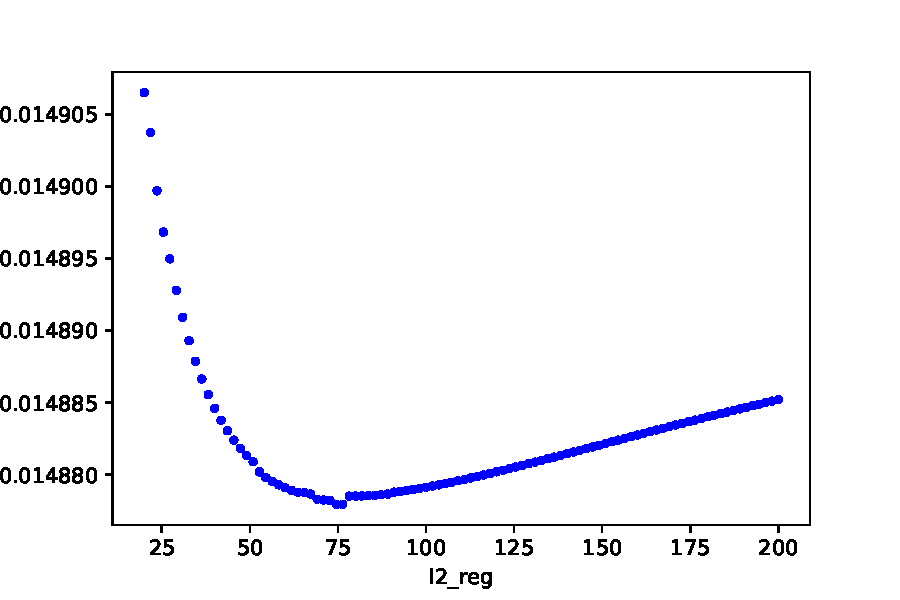
\includegraphics[width=.6\textwidth]{MSE_l2_dependency_0_filtering.pdf}\hfill
		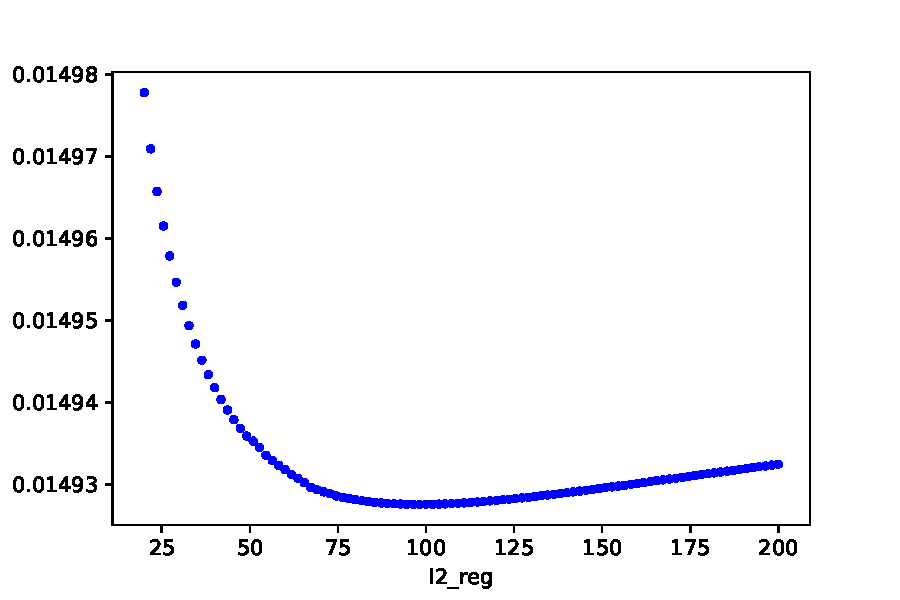
\includegraphics[width=.6\textwidth]{MSE_l2_dependency_10_filtering.pdf}\hfill
		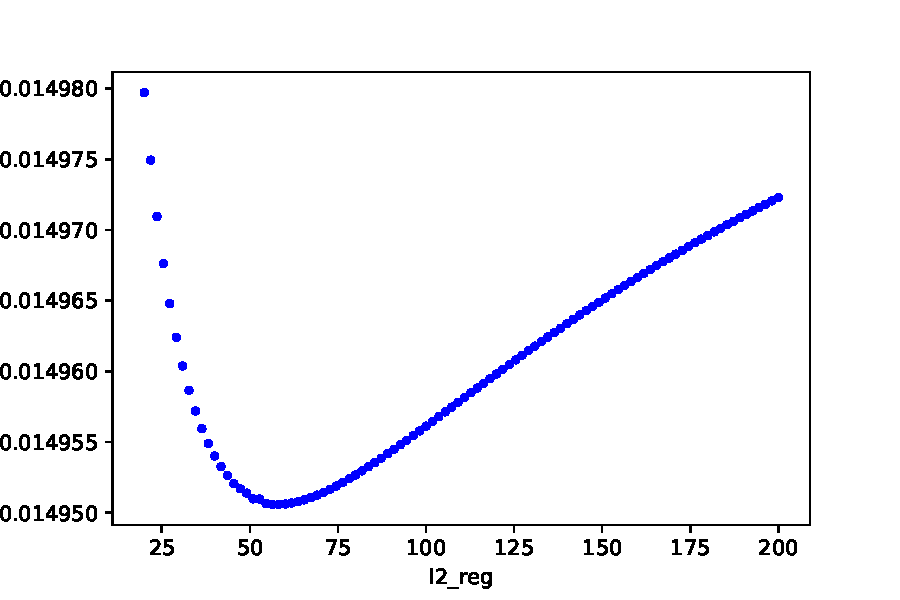
\includegraphics[width=.6\textwidth]{MSE_l2_dependency_15_filtering.pdf}
		
		\caption{Зависимость MSE от l2-регуляризации. На первом рисунке график строится для данных без удаления шума, на втором с удалением 10\% шума, на третьем --- 15. На всех графиках critical p-value=90}
		\label{fig:mse_l2}
	\end{figure}
	
	Для чего нужны полученные оценки на параметры? Они нужны для того, чтобы определять наиболее устойчивые метрики путём проведения множества "случайных" экспериментов. При этом устойчивость будет определяться количеством экспериментов, в которых вес сохранял знак. Таким образом можно будет выявить метрики, которые стабильно одного знака в разных условиях, из чего можно будет сделать вывод, что они влияют на изучаемую таргет-метрику строго определённым образом -- увеличивают или уменьшают. \\
	
	Для определения этого удобнее использовать графическую интерпретацию, потому что важно не только количество "отклонений" от мажорирующего направления, но и насколько сильным оно было. Такая интерпретация представлена на рисунке \ref{fig:0_metric_stability}. Такие графики можно построить для всех остальных long-term метрик.
	
	\begin{figure}
		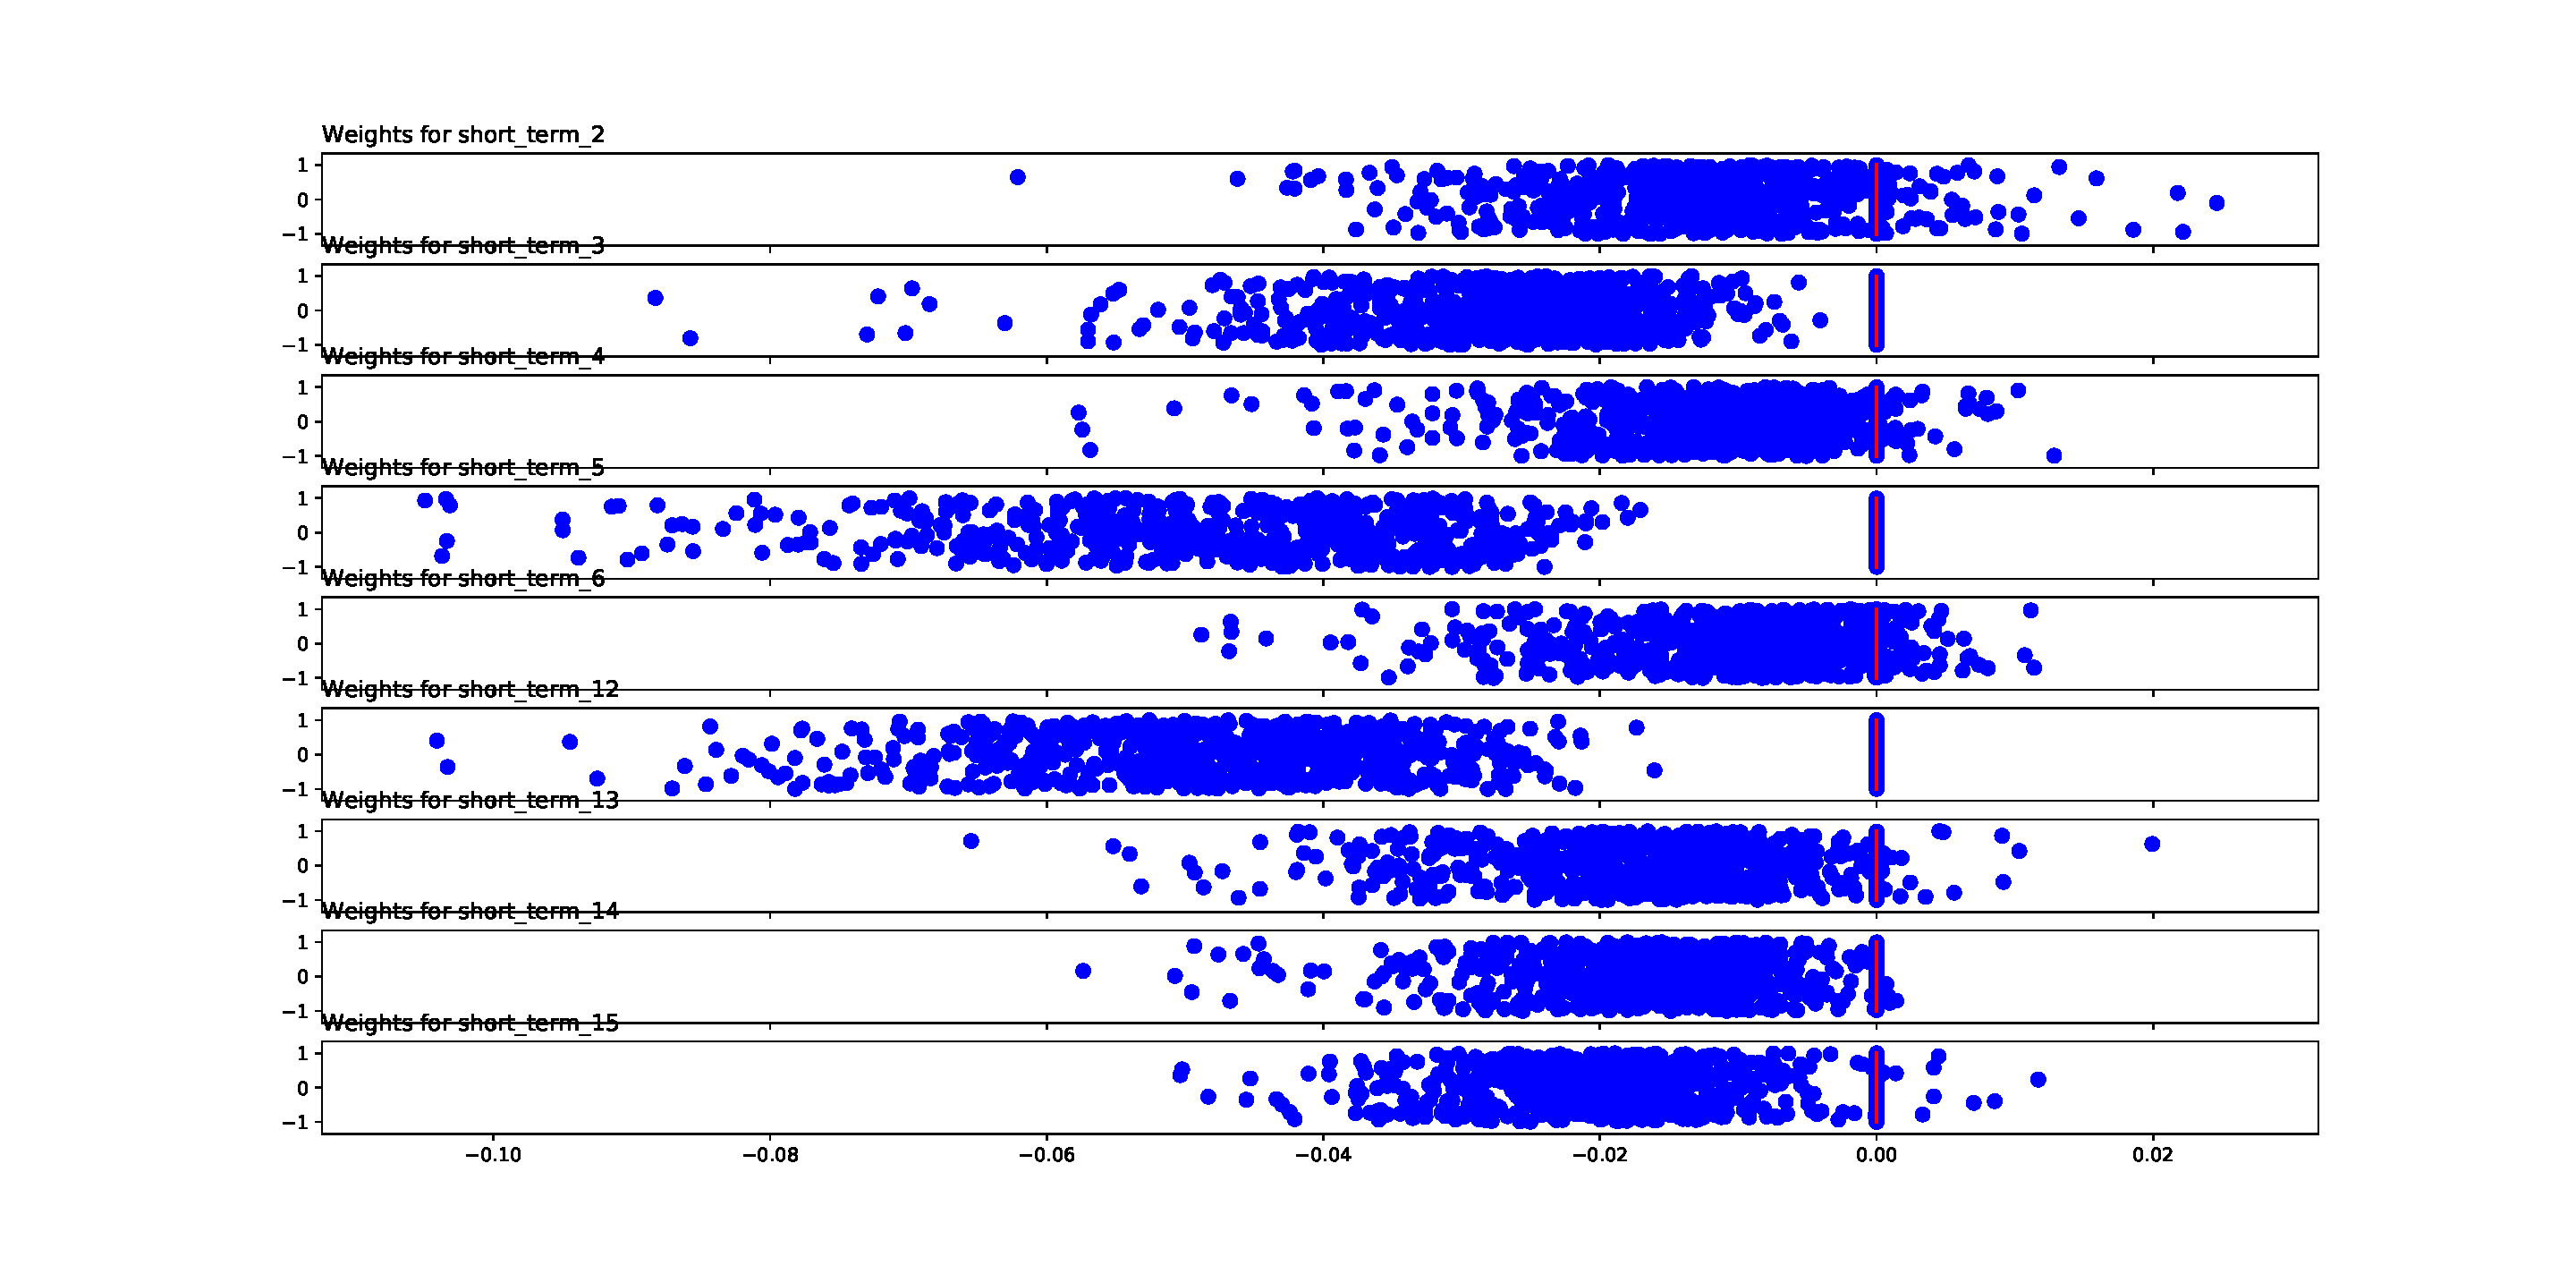
\includegraphics[scale=0.4]{0_metric_stability.pdf}
		\caption{Зависимость long-term-0 от коротких метрик. Здесь изображены только те метрики, у которых мажорирующий знак встречается хотя бы в 80\% экспериментов. График стоит рассматривать как график на прямой, а не на плоскости, вторая ось была сделана только для наглядного отображения "плотности" скопления точек. Из такого графика можно сделать вывод, что 3, 5, 12 метрики -- очень устойчивы. Так же, 14 метрика вызывает доверие. В остальных случаях можно поисследовать случаи смены знака, но в любом случае эти метрики будут менее стабильными.}
		\label{fig:0_metric_stability}
	\end{figure}


	
\end{document}